\chapter{Introdução}\label{introducao}
% determinacao da potencia sonora
Várias técnicas de controle de ruído foram desenvolvidas nesses últimos tempos visando oferecer ao ouvido humano um ambiente agradável, principalmente no que diz respeito a filtragem em determinadas faixas de frequências. Para tanto, faz-se uso de filtros acústicos de natureza mecânica.

Para a determinação dos procedimentos de medição da perda de transmissão de filtros acústicos tomasse como referência a norma ASTM E2611 – 9 Standard Test Method for Measurement of Normal Incidence Sound Transmission of Acoustical Materials Based on the Transfer Matrix Method. Os procedimentos descritos nessa norma abrange a utilização de um tubo, quatro microfones, um hardaware para aquisição do sinal em níveis de pressão e um software de análise de sinal para a determinação das funções de transferência e outras propriedades acústicas relevantes.

Em vista do que foi exposto, esse trabalho tem como objetivo determinar e analisar o comportamento da absorção acústica em dois tipos de filtros acústico: câmara de expansão e ressonador de Helmholtz.

\chapter{Fundamentação Teórica}\label{fundamentacao}

\section{Tubo com Ressonador de Helmholtz}

Considere um ressonador de Helmholtz, como o mostrado na figura \ref{fig.ressonador}, com volume $V$, pescoço de comprimento $L$ e seção transversal $S$.

\begin{figure}[h]
\centering
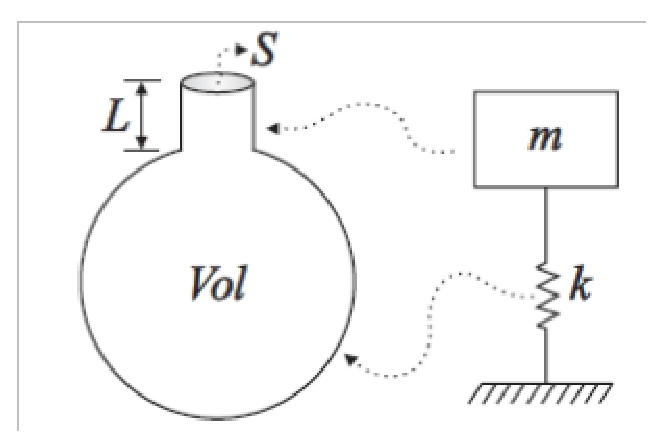
\includegraphics[scale=0.45]{ressonador.eps}
\caption{Exemplo de ressonador}
\label{fig.ressonador}
\end{figure}

O gás contido no pescoço possui uma massa efetiva:
\begin{equation}
    m = \rho_{0}SL
\end{equation}

A rigidez do sistema é dado por:
\begin{equation}
    K = \frac{-\rho_{0}c^{2}_{0}S^{2}}{V}
\end{equation}

Analisando o ressonador como um sistema de um grau de liberdade, pode-se calcular a frequência de ressonância, dada através da equação de movimento (sem dissipação e sem excitação). A ressonância ocorre quando:

\begin{equation}
    f_{0} = \frac{c_{0}}{2\pi}\sqrt{\frac{S}{LV}} [Hz]
\end{equation}

\newpage
As dimensões do ressonador empregado no estudo são dadas na figura \ref{ressonador_2}.
\begin{figure}[h]
\centering
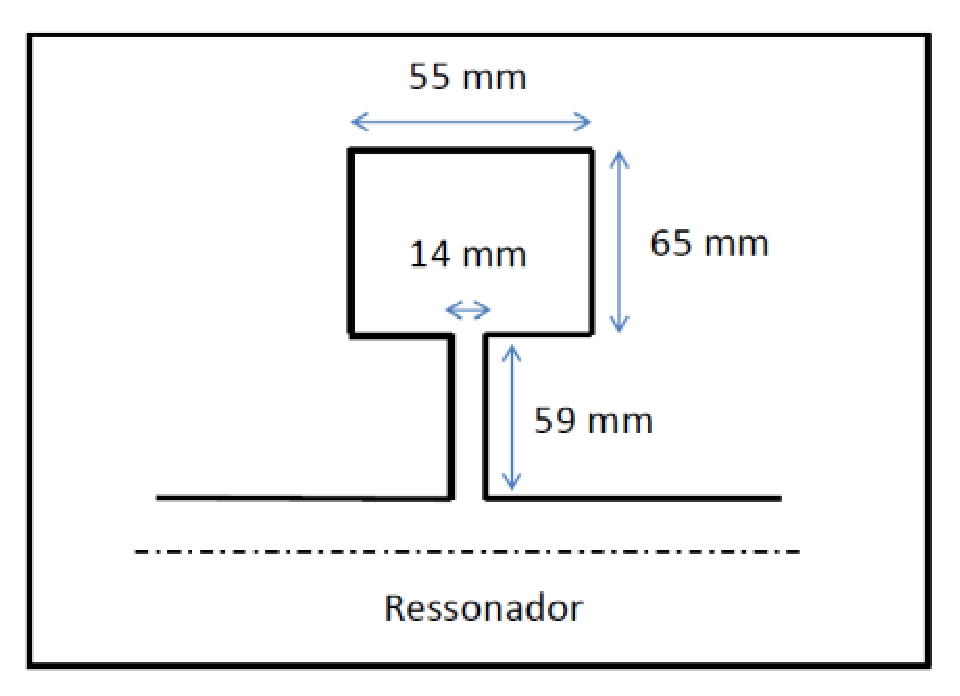
\includegraphics[scale=0.45]{ressonador_2.eps}
\caption{Ressonador abordado no estudo.}
\label{ressonador_2}
\end{figure}

\section{Câmara de Expansão}

Considere um tubo de seção transversal $S1$ contendo uma câmara de expansão de área $S2$ representado na figura \ref{camara}.
\begin{figure}[h]
\centering
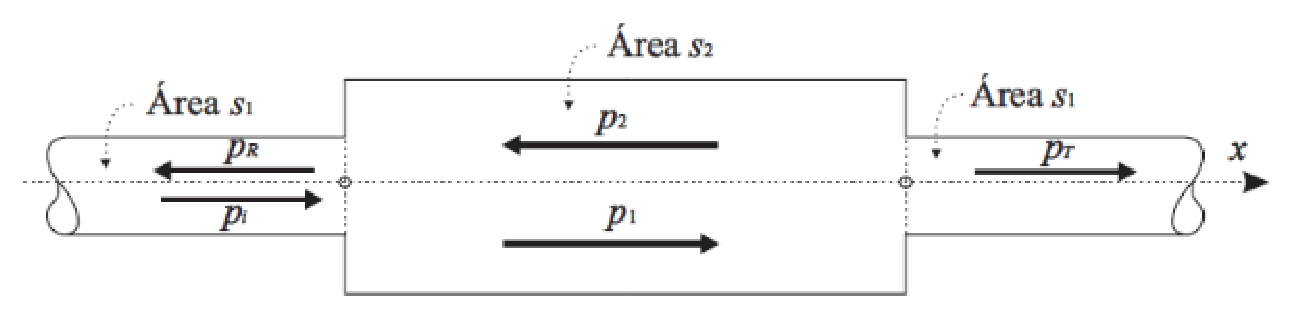
\includegraphics[scale=0.45]{camara.eps}
\caption{Câmara de expansão.}
\label{camara}
\end{figure}

Rearranjando as equações que descrevem o movimento de uma onda pelo tubo e aplicando as devidas condições de contorno, pode-se chegar à razão entre a potência transmitida e a incidente. Para isso, necessita-se determinar a razão $P_{t}/P_{i}$ e a razão $W_{trans}/W_{incid}$ fica:
\begin{equation}
    \frac{W_{trans}}{W_{incid}} = \frac{S_{1}P_{t}^{2}}{S_{1}P_{i}^{2}} = \frac{S_{1}\frac{P_{t}^{2}}{\rho_{0}c_{0}}}{S_{1}\frac{P_{i}^{2}}{\rho_{0}c_{0}}}
\end{equation}

Obtendo-se assim o coeficiente de transmissão $\alpha_{t}$:
\begin{equation}
    \alpha_{t} = \frac{P_{t}^{2}}{P_{i}^{2}} = \frac{4}{4cos^{2}(kl)+(\frac{S_{2}}{S_{1}}+\frac{S_{1}}{S_{2}})^{2}sen^{2}(kl)}
\end{equation}

E a perda de transmissão é dada por:
\begin{equation}
    TL = 10log(\frac{I_{trans}}{I_{incid}})^{-1} = 10log(\alpha_{t})^{-1}
\end{equation}

Câmaras de expansão proporcionam atenuação ao longo de amplas faixas de frequência (Figura 2). Maiores atenuação são obtidas quanto maior a razão entre as áreas $S_{1}/S_{2}$. O coeficiente de transmissão $\alpha_{t}$ apresenta valores unitários para frequências tais que $sen(kl) = 0$, ocorrendo quando:
\begin{equation}
    L = n\frac{\lambda}{2}
\end{equation}
Tal que $n = 1,2,3...$.

As máximas atenuações ocorrem quando $cos(kl) = 0$, e isto ocorre quando:
\begin{equation}
    kL = n\frac{pi}{2}
\end{equation}
Tal que $n = 1,3,5 ...$

Este modelo considera apenas as ressonâncias formadas na direção axial da câmara. Na prática, ocorrem formações de ondas estacionárias nas demais direções também (radial e circunferencial, se a cavidade for cilíndrica). Para nossos testes foi empregado a câmara de expansão ilustrada na figura \ref{camara_2}.

\begin{figure}[h]
\centering
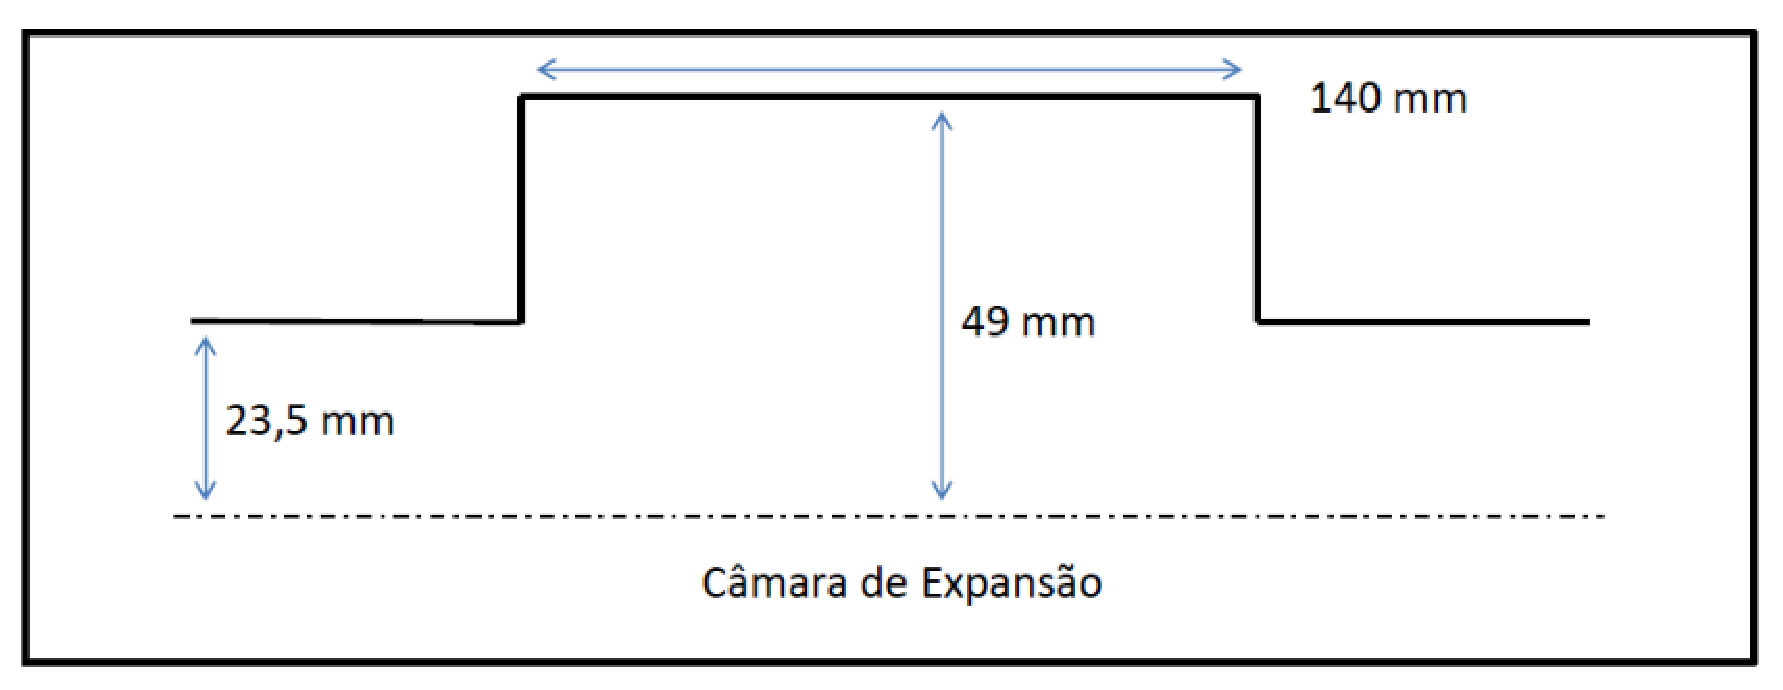
\includegraphics[scale=0.32]{camara_2.eps}
\caption{Câmara de expansão abordada no estudo.}
\label{camara_2}
\end{figure}

\chapter{Experimento}\label{descricao}

O experimento consiste de dois tubos com área interna iguais que possam ter umas das suas extremidades unidas por um tubo porta amostra (tubo onde a amostra é inserida). O número de conjuntos de tubo dependerá do range de frequência a ser testado. Numa das extremidades do tubo há uma caixa de som e na outra uma terminação anecóica \ref{tubo}.

\begin{figure}[h]
\centering
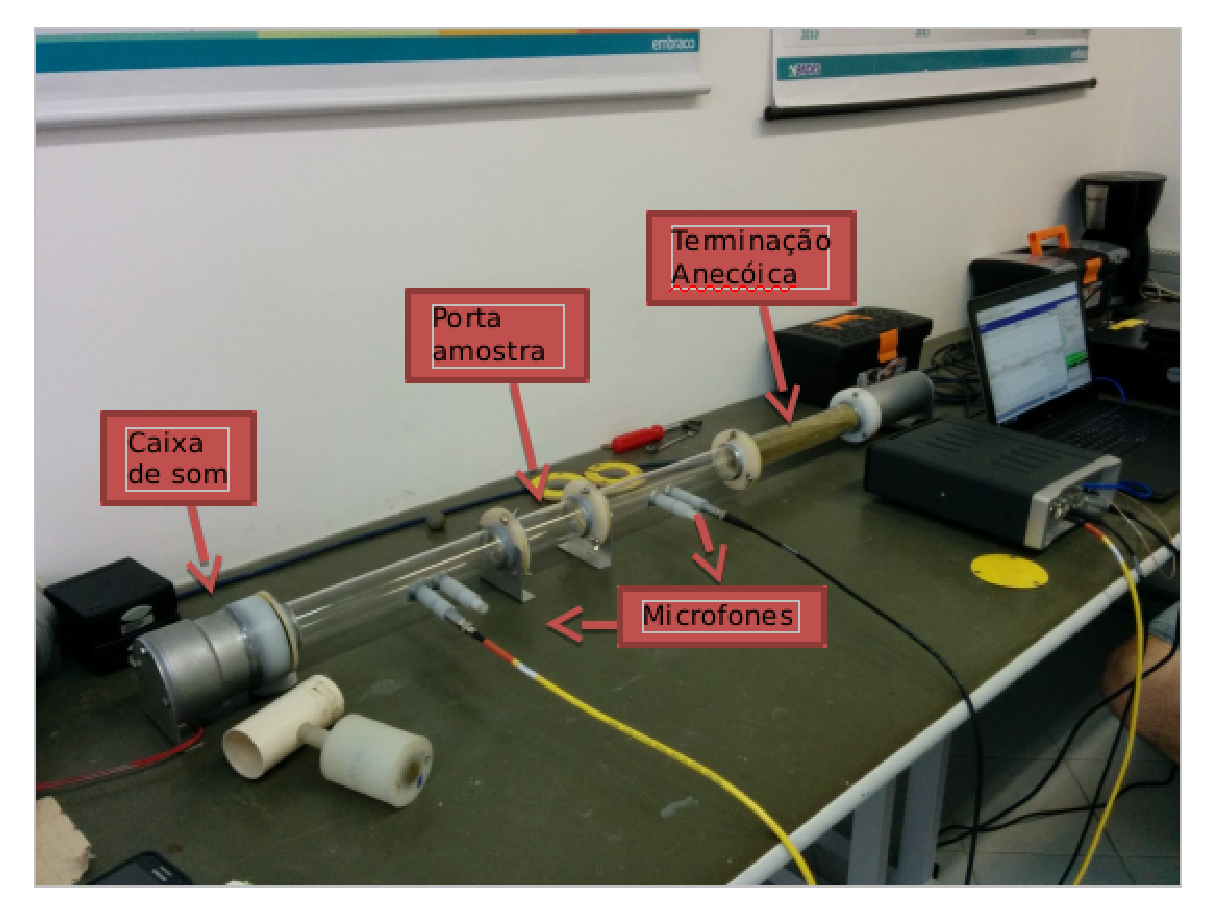
\includegraphics[scale=0.72]{tubo.eps}
\caption{Tubo para o experimento.}
\label{tubo}
\end{figure}

A frequência mínima é determinada pelo espaço entre os microfones e a precisão do sistema de aquisição de dados. O espaço entre os microfones deve ser maior que um por cento do comprimento de onda correspondente da menor frequência de interesse. Em nosso experimento a distância entre o dois primeiros microfones é de 31,5mm e dos segundos microfones é de 30,0 mm.

A frequência máxima depende do diâmetro do tubo, o espaço entre os microfones, da velocidade do som e pode ser calculada por:
\begin{equation}
    f_{max} < \frac{Kc}{d}
\end{equation}
Tal que $f_{max}$ é a frequência máxima, $c$ é a velocidade do som no tubo (m/s), $d$ é o diâmetro do tubo (m) e $K$ uma constante no valor de 0.856.

Posicionado no lado esquerdo estará o a fonte sonora, que deverá ter uma reposta plana no range de frequência de interesse. Podendo ser coaxial com o tubo principal ou unido ao tubo principal por meio de uma união exponencial (tipo corneta). O sinal empregado nos testes deverá ser um sinal aleatório tendo uma densidade espectral uniforme ao longo da frequência de interesse. Em nossos testes foi utilizado um ruído branco pseudoaleatório.
No lado direito do tubo será instalado uma terminação anecóica. Uma conveniente maneira de obter essa terminação é instalar uma espuma isolante, tipo lã de rocha ou fibra de vidro, de forma piramidal de 30 cm de comprimento no final do tubo.
 A obtenção dos dados dá-se por meio da determinação da matriz de transferência, que por sua vez será obtida a partir de três medições da função transferência $H$. Serão realizados três testes para o ressonador de Helmholtz e três para a câmara de expansão com dois tipos diferentes de terminação, anecóica e rígida. Além disso serão realizados também três testes com o tubo vazio para as duas terminações anecóica e rígida, para encontrar a curva de perda de transmissão do tubo sem nenhum material dentro.

\chapter{Resultados}\label{resultados}

\begin{figure}[h]
%\centering
\hspace{-4.5cm}
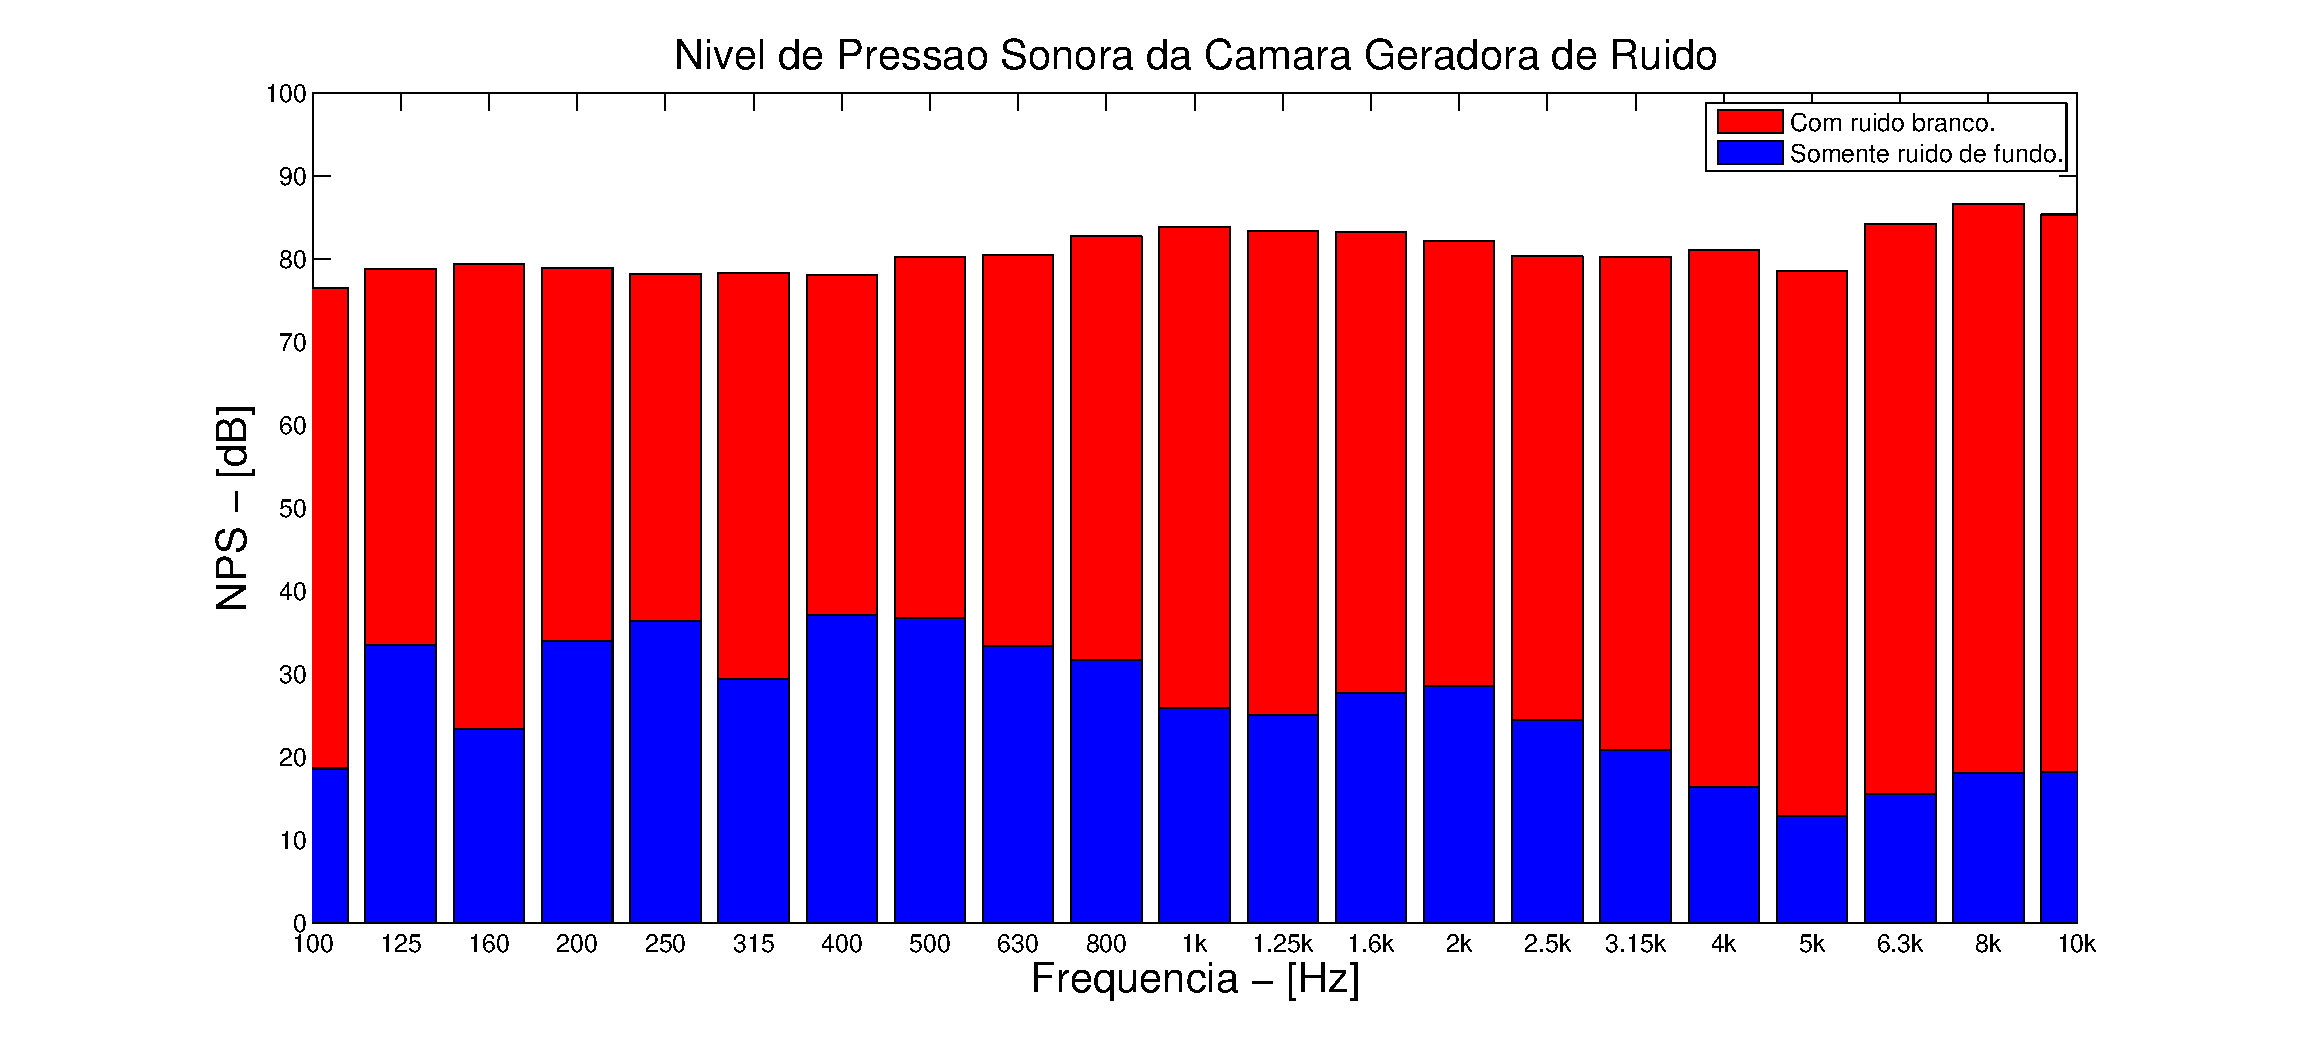
\includegraphics[scale=0.6]{codigo/pressao_sonora_geradora.eps}
%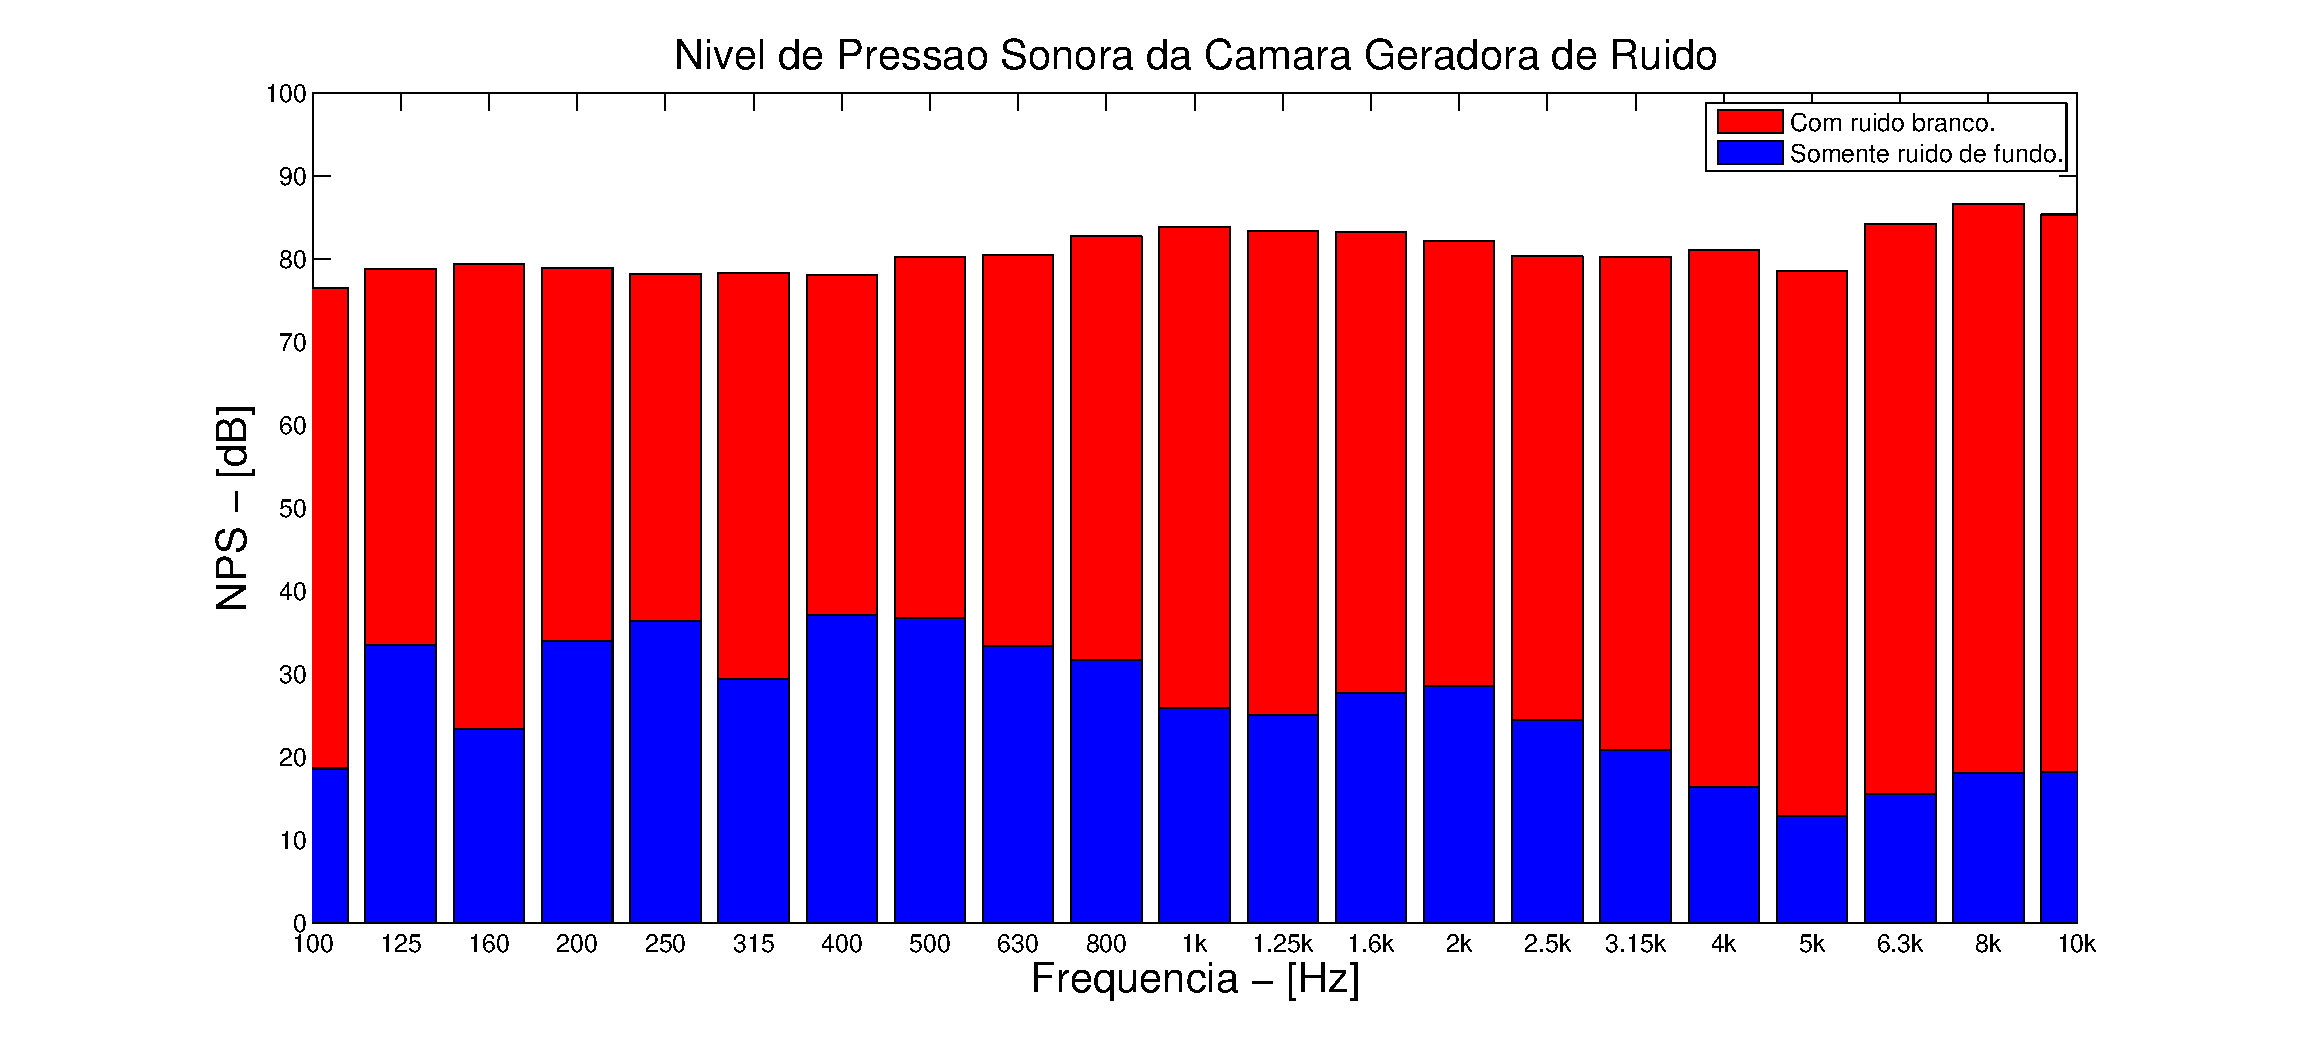
\includegraphics[width=40cm,height=40cm,keepaspectratio]{codigo/pressao_sonora_geradora.eps}
\caption{Níveis de pressão sonora na câmara geradora de ruído branco.}
\label{resultado_1}
\end{figure}


\begin{figure}[h]
%\centering
\hspace{-4.5cm}
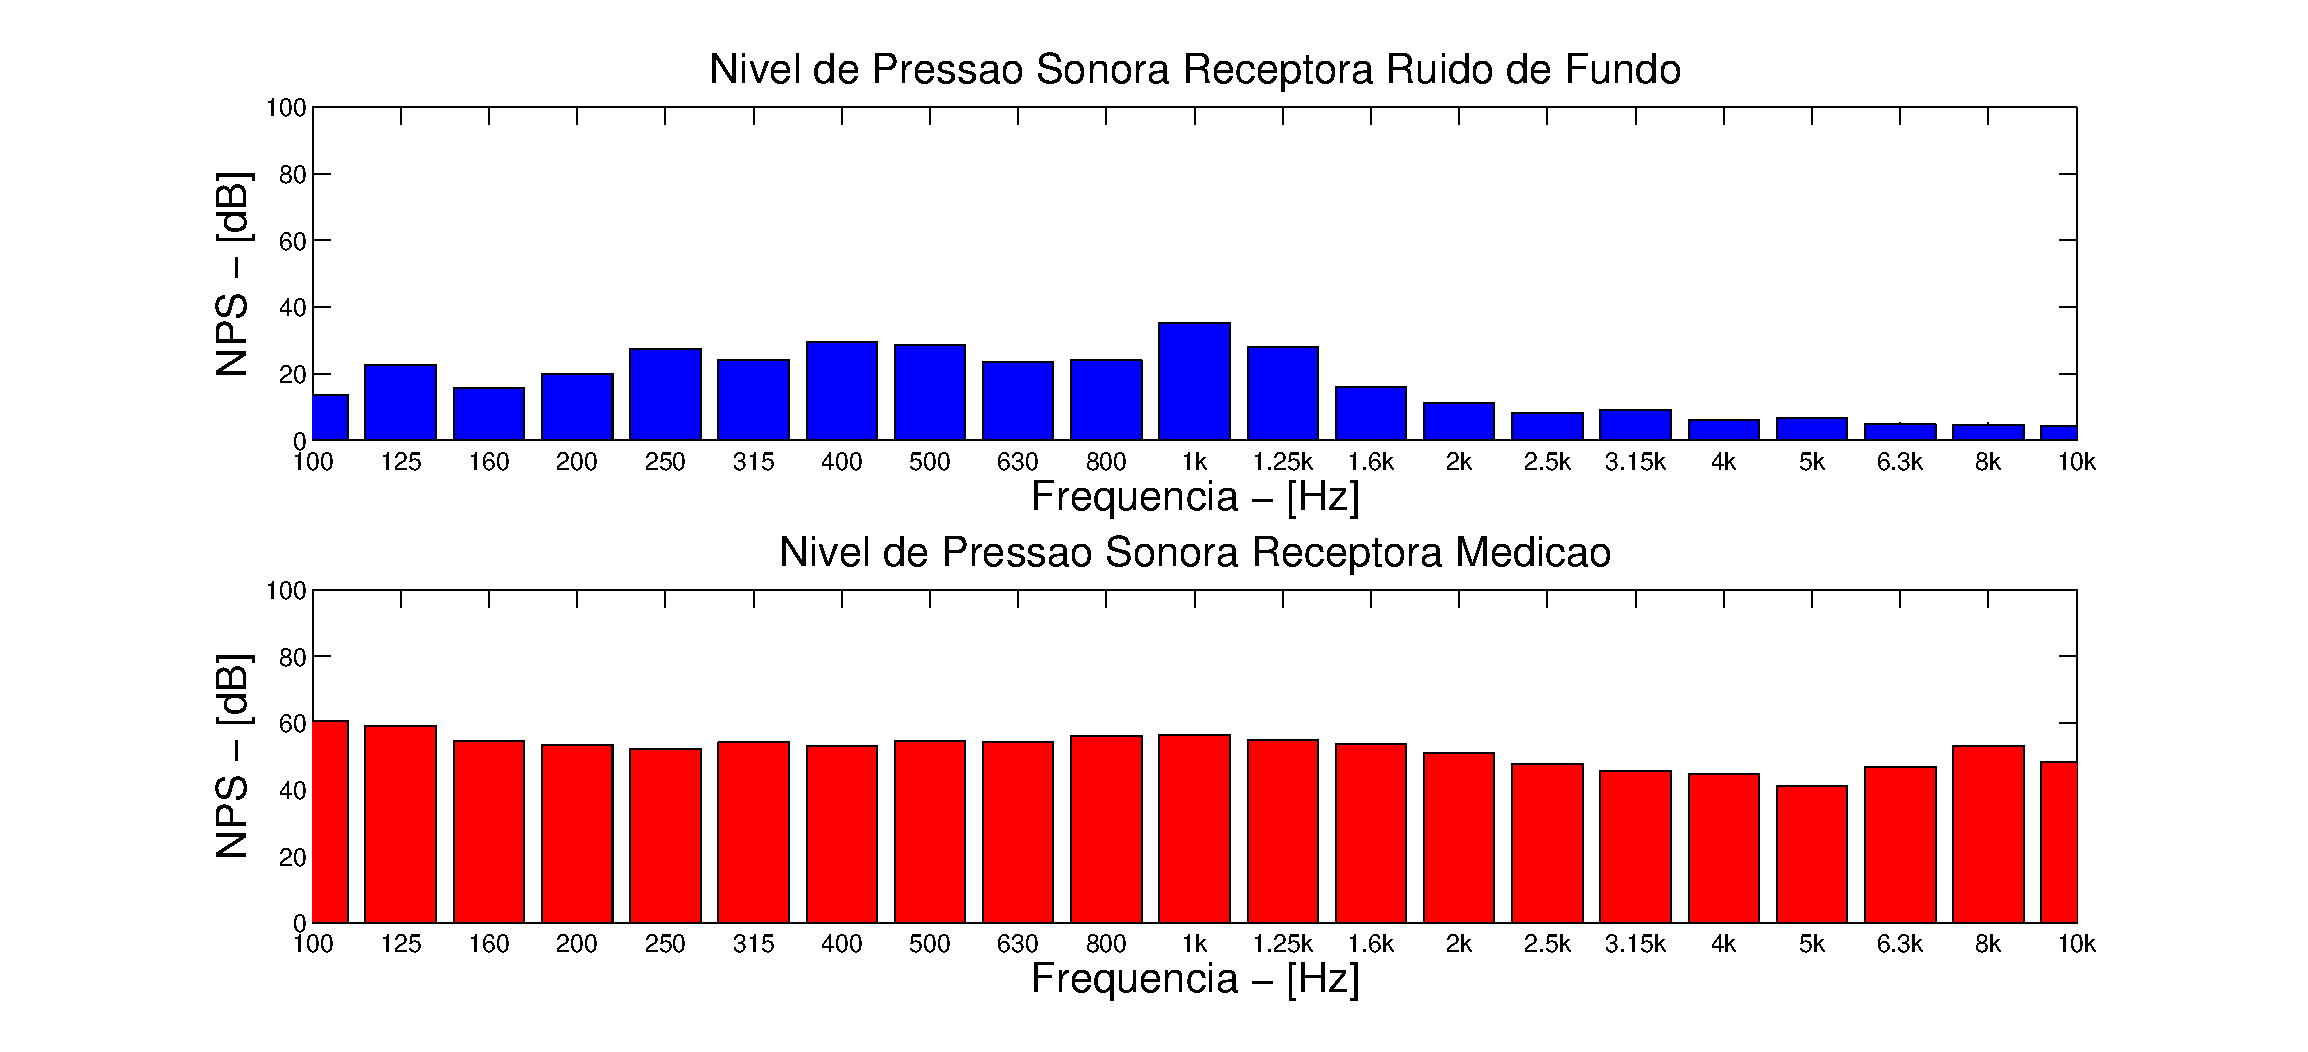
\includegraphics[scale=0.6]{codigo/pressao_sonora_receptora.eps}
\caption{Níveis de pressão sonora na câmara receptora de ruído branco.}
\label{resultado_2}
\end{figure}

\begin{figure}[h]
%\centering
\hspace{-4.5cm}
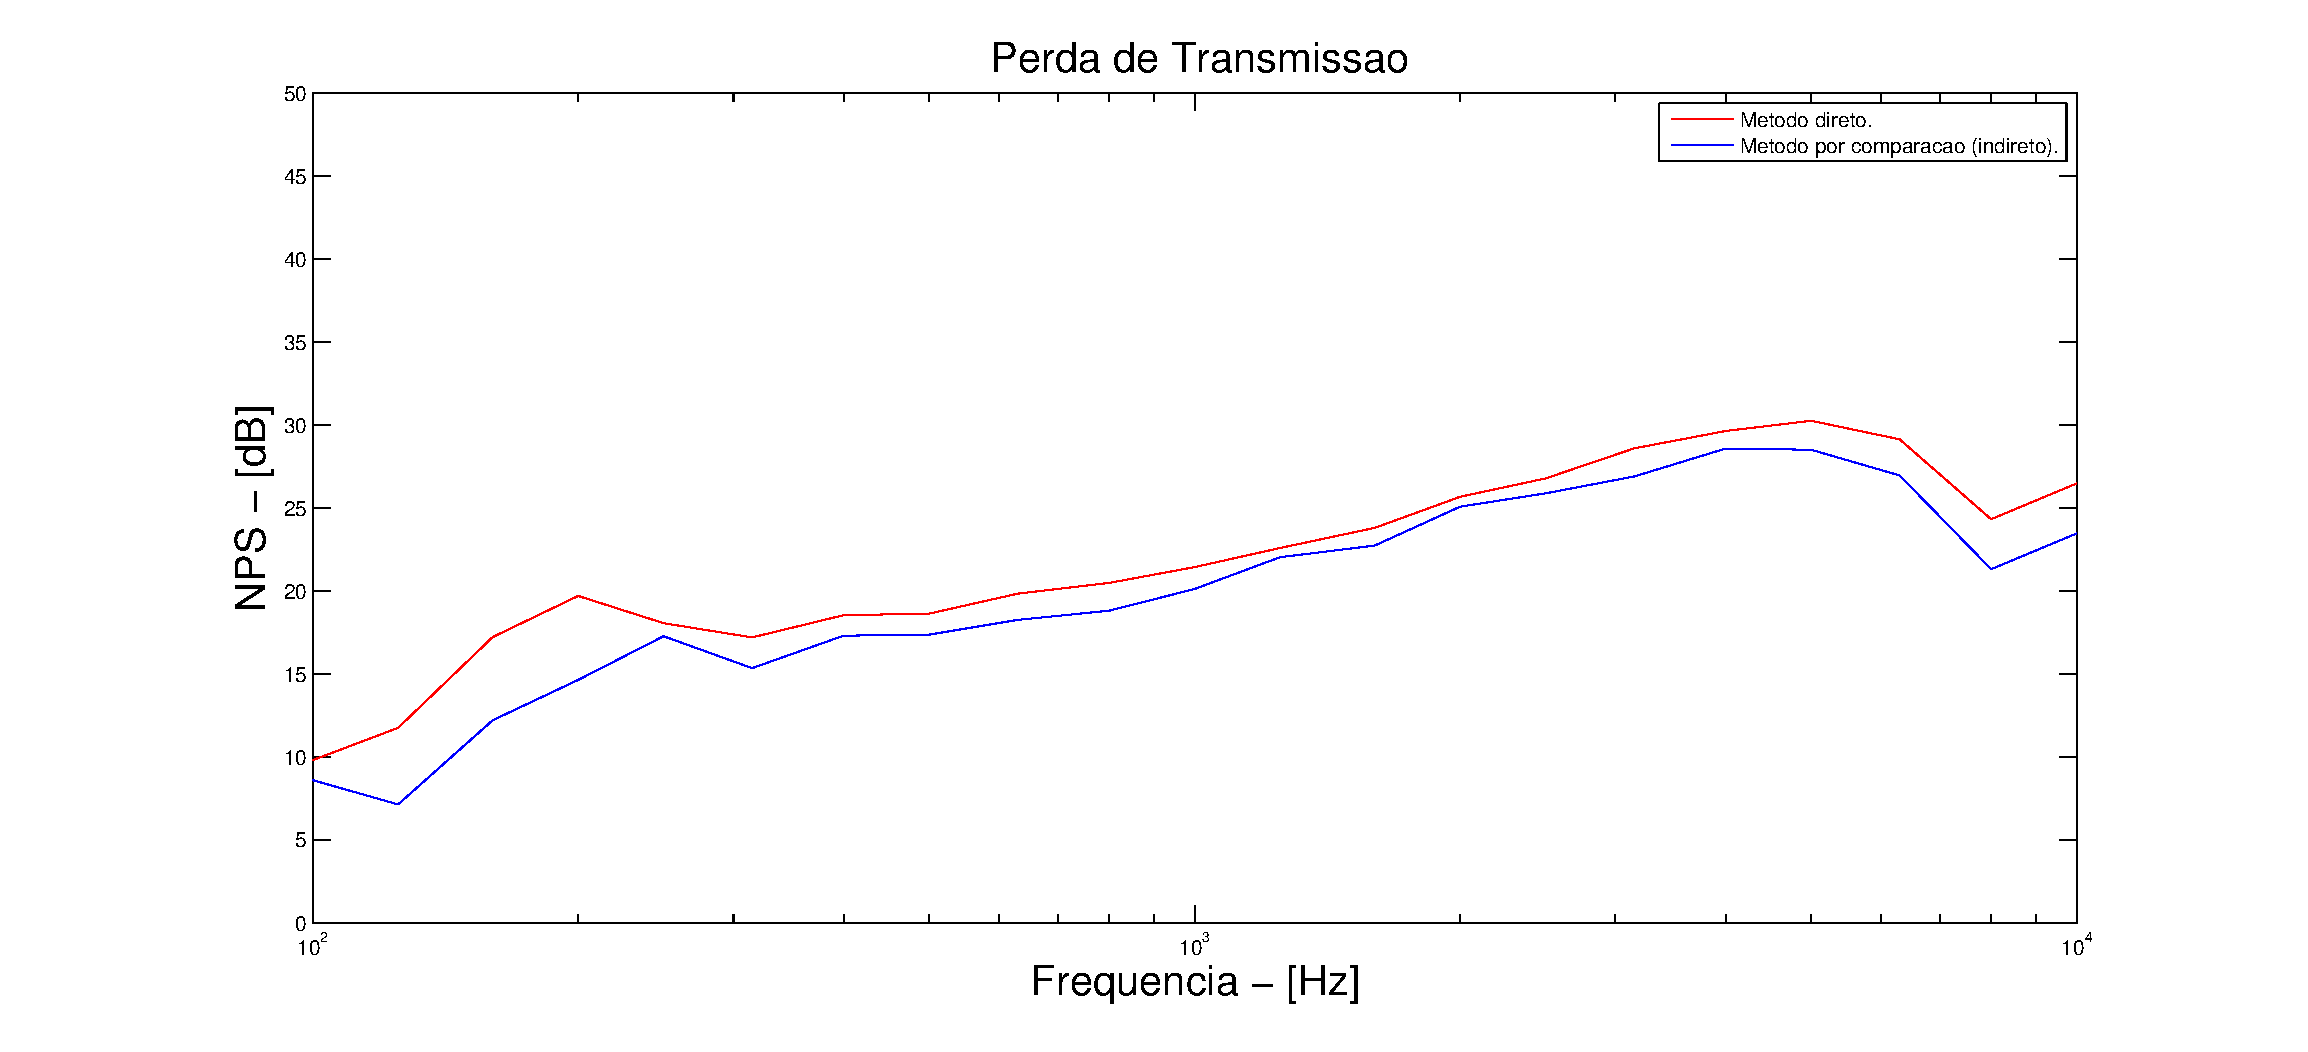
\includegraphics[scale=0.6]{codigo/perda_transmissao.eps}
\caption{Gráfico de perda de transmissão da placa de alumínio.}
\label{resultado_3}
\end{figure}


\chapter{Conclusões}\label{conclusoes}

O experimento descrito anteriormente reforçou as particularidades do uso da câmara de expansão e do ressonador de Helmholtz frente a perda de transmissão. Observa-se que o ressonador de Helmholtz atua como uma solução precisa e pontual, atuando em uma determinada frequência única. Ao contrário da câmara de expansão, que atua em uma faixa larga de frequência. No entanto esta última deve ser projetada para que os maiores níveis de atenuação ocorram nas frequências que deseja-se, caso contrário pode-se encontrar um anti-pico na curva e sua utilização não ter efeito nenhum de atenuação(1296 Hz, 2524 Hz e 3810 Hz).